\documentclass[12pt]{article}
\usepackage[spanish]{babel}
\usepackage{geometry}
\usepackage{graphicx}
\usepackage{setspace}
\usepackage{hyperref}
\usepackage{apacite}
\usepackage{fancyhdr}
\usepackage{titlesec}
\usepackage{nopageno}


%  small letter size for title 12fnt
%     key words in the footer
%  resumen: falta la problematica y definir, gstacion de los recursos/luz, sobra muchas cosas que no hicimos, ong, organismos gobernanmntales, hab
\geometry{a4paper, margin=1in}
\doublespacing
\title{\large{\textbf{AquaSolar: Sistema de Riego Sostenible para Huertas}}}
\author{Juan Andrés Del Toro R, Nathan Alspaugh y Juan Pablo Ortiz \\ Medioambiente, Colegio Real Royal School \\ 11 Grado \\ Lic. Corina Corpas Santofimio \\ 2025}
\date{}
\begin{document}
\pagestyle{fancy}
\cfoot{}
\fancyhead{} % clear all header fields
\fancyhead[LO,CE]{\textbf{AquaSolar:  Sistema de Riego Sostenible para Huertas
      }}
\fancyhead[RO,RO]{\thepage}
\maketitle

\newpage
\renewcommand{\thesection}{}
\renewcommand{\thesubsection}{}
\renewcommand{\thesubsubsection}{}
\titleformat{\section} % Command to modify
{\normalfont\Large\bfseries} % Font style for the section title
{\thesection} % Section number (optional)
{0pt} % Space between number and title
{} % Code before the title (optional)

% Customize subsection formatting
\titleformat{\subsection} % Command to modify
{\normalfont\large\bfseries} % Font style for the subsection title
{\thesubsection} % Subsection number (optional)
{1em} % Space between number and title
{} % Code before the title (optional)

% Customize subsubsection formatting
\titleformat{\subsubsection} % Command to modify
{\normalfont\normalsize\bfseries} % Font style for the subsubsection title
{\thesubsubsection} % Subsubsection number (optional)
{2em} % Space between number and title
{} % Code before the title (optional)
\newpage
\section*{Resumen}
El acceso al agua potable ha sido históricamente un desafío para la humanidad. Desde las primeras civilizaciones, como los sumerios y egipcios, quienes desarrollaron avanzados sistemas de irrigación y acueductos, hasta la actualidad, la gestión del agua ha sido crucial para el desarrollo de las sociedades. En este contexto, el proyecto Aqua Solar propone una solución innovadora basada en la integración de tecnologías fotovoltaicas en sistemas de captación, purificación y distribución de agua potable. Su objetivo principal es garantizar un suministro continuo y sostenible de agua en comunidades con infraestructura deficiente, reduciendo la dependencia de fuentes de energía convencionales.

La metodología del proyecto combina estudios de impacto ambiental, diseño de prototipos y pruebas en entornos reales. Se espera desarrollar un sistema autosustentable, capaz de operar en zonas con recursos limitados, mejorando la calidad de vida de las poblaciones beneficiarias. La duración estimada es de 12 meses, incluyendo las fases de investigación, desarrollo e implementación. Para su ejecución, se requiere la instalación de paneles solares, sistemas de filtración avanzada y un modelo de distribución eficiente. El proyecto beneficiará tanto a comunidades rurales con acceso limitado al agua como a organismos gubernamentales y ONGs interesadas en promover soluciones ecológicas. A largo plazo, Aqua Solar busca sentar un precedente en la gestión sostenible del recurso hídrico, alineado con los Objetivos de Desarrollo Sostenible (ODS) de las Naciones Unidas.
\newpage
\section*{Abstract}
Access to clean water has historically been a challenge for humanity. From early civilizations, such as the Sumerians and Egyptians, who developed advanced irrigation systems and aqueducts, to the present day, water management has been crucial to the development of societies. In this context, the Aqua Solar project proposes an innovative solution based on integrating photovoltaic technologies into systems for collecting, purifying, and distributing potable water. Its primary goal is to ensure a continuous and sustainable water supply for communities with inadequate infrastructure, reducing reliance on conventional energy sources.

The project’s methodology combines environmental impact studies, prototype design, and real-world testing. The aim is to develop a self-sustaining system capable of operating in resource-limited areas, improving the quality of life for beneficiary populations. The estimated timeline is 12 months, including research, development, and implementation phases. Execution requires installing solar panels, advanced filtration systems, and an efficient distribution model. The project will benefit both rural communities with limited water access and government agencies or NGOs interested in promoting eco-friendly solutions. Long-term, Aqua Solar aims to set a precedent for sustainable water resource management, aligning with the United Nations’ Sustainable Development Goals (SDGs).
\newpage
\renewcommand{\contentsname}{Tabla de Contenido}
\tableofcontents


\newpage
\section{Justificación}
El agua es el recurso más vital para la humanidad, pero su acceso equitativo sigue siendo un reto global. Según el Informe Mundial de las Naciones Unidas sobre el Desarrollo de los Recursos Hídricos (2021), más de 2.200 millones de personas carecen de acceso seguro a agua potable. Este problema se agudiza en comunidades con limitaciones en infraestructura, donde las fuentes hídricas suelen ser escasas o están contaminadas por agentes biológicos y químicos.

Históricamente, diversas civilizaciones han enfrentado crisis hídricas que han determinado su sostenibilidad. Un caso emblemático es la civilización maya, que dependía de reservorios de agua de lluvia llamados chultunes; la sequía prolongada y la falta de tecnología adecuada para la gestión del agua fueron factores clave en su colapso. Actualmente, la crisis climática plantea desafíos similares, intensificando la desertificación y reduciendo la disponibilidad del recurso.

El proyecto Aqua Solar surge como una alternativa innovadora para enfrentar esta crisis, utilizando la energía solar como fuente de abastecimiento energético para el tratamiento y distribución del agua. La justificación de su implementación se basa en tres pilares fundamentales:

Sostenibilidad energética y ambiental: El uso de energía fotovoltaica reduce la huella de carbono y elimina la dependencia de combustibles fósiles en los procesos de captación y purificación del agua. Esto es especialmente relevante en países en desarrollo, donde la infraestructura eléctrica es ineficiente y costosa.

Impacto en la salud pública: Las enfermedades de origen hídrico, como el cólera y la diarrea, siguen siendo una de las principales causas de mortalidad en regiones con acceso limitado al agua potable. Al implementar un sistema seguro de abastecimiento, Aqua Solar contribuirá a la reducción de enfermedades transmitidas por el consumo de agua contaminada.

Viabilidad económica y replicabilidad: Si bien la inversión inicial en infraestructura fotovoltaica puede ser elevada, los costos operativos son significativamente bajos a largo plazo. Además, el modelo de Aqua Solar está diseñado para ser escalable y adaptable a diversas condiciones geográficas, permitiendo su implementación en distintas regiones con necesidades similares.

\newpage
\section{Introducción}
Desde tiempos ancestrales, la humanidad ha desarrollado sistemas para gestionar el agua, desde los sofisticados acueductos romanos hasta las represas modernas. Sin embargo, a pesar de estos avances, la crisis del agua sigue siendo una de las problemáticas más urgentes del siglo XXI. El crecimiento demográfico, el cambio climático y la sobreexplotación de los recursos hídricos han llevado a un punto crítico en el cual la innovación tecnológica es indispensable para garantizar el acceso equitativo a este recurso.

Aqua Solar es un proyecto que nace en respuesta a esta crisis, proponiendo una solución basada en la integración de energía solar en sistemas de abastecimiento de agua potable. Su enfoque se centra en la implementación de tecnología fotovoltaica para la captación, filtración y distribución del recurso hídrico en comunidades con infraestructura limitada. El campo de estudio de este proyecto abarca la ingeniería ambiental, la gestión de recursos hídricos y las energías renovables, combinando estos conocimientos para desarrollar una solución eficiente y sostenible.

Diversos estudios han demostrado la eficacia del uso de energía solar en el bombeo y purificación del agua. Un ejemplo relevante es el caso de India, donde proyectos piloto han demostrado que los sistemas fotovoltaicos pueden reducir en un 70\% los costos operativos del suministro de agua en zonas rurales (World Bank, 2020). Inspirado en estos modelos de éxito, Aqua Solar busca adaptar estas soluciones a comunidades latinoamericanas con condiciones climáticas similares, optimizando su eficiencia y accesibilidad.

El desarrollo de este proyecto se basa en tres etapas fundamentales: investigación y diseño, construcción de prototipos y pruebas en campo. Se identifican desafíos como la variabilidad de la radiación solar, el costo de mantenimiento y la necesidad de formación técnica para los usuarios. No obstante, se han diseñado estrategias para mitigar estos riesgos, como el uso de baterías de almacenamiento energético y la capacitación comunitaria.
\newpage
\section{Planteamiento del problema}
\subsection{Tema}
Diseño e Implementación de un Sistema de Riego Sostenible para Huertas, Utilizando Energía Solar para Maximizar la Eficiencia en el Uso del Agua y Reducir el Impacto Ambiental.

\subsection{Pregunta Problema}
¿Cómo aprovechar de manera eficiente la energía solar para automatizar el riego en huertas, maximizando el uso del agua y reduciendo los costos operativos, mientras se minimiza el impacto ambiental?
\newpage
\section{Objetivos}
\subsection{Objetivo General}
Diseñar e implementar un sistema de riego automatizado para huertas, alimentado por energía solar, con el propósito de optimizar el uso del agua, reducir el consumo de energía y promover prácticas agrícolas sostenibles.

\subsection{Objetivos Específicos}
\begin{itemize}
      \item Desarrollar un controlador automático de riego que ajuste la cantidad y frecuencia del agua de acuerdo con las necesidades específicas de las plantas.
      \item Integrar paneles fotovoltaicos para alimentar el sistema de riego, disminuyendo la huella de carbono y la dependencia de energías no renovables.
      \item Medir la eficiencia del sistema en términos de ahorro de agua y energía, evaluando su viabilidad económica para la institución.
      \item Fomentar la sostenibilidad ambiental y la educación sobre energías renovables, estableciendo un modelo replicable para otras huertas educativas.
\end{itemize}
\newpage
\section{Marco Teórico}
\subsection{Introducción al Riego Sostenible}
El riego sostenible se refiere al uso racional del agua, con el objetivo de minimizar su desperdicio y reducir el impacto ambiental. En este proyecto, la energía solar es utilizada para implementar un sistema de riego automatizado en huertas escolares, promoviendo el ahorro de recursos y contribuyendo a la educación ambiental de los estudiantes.

\subsection{Conceptos Clave}
\begin{itemize}
      \item \textbf{Energía Solar}: Obtenida a través de paneles fotovoltaicos, convierte la luz solar en electricidad, lo cual permite una fuente de energía renovable y libre de emisiones para el riego.
      \item \textbf{Automatización del riego}: Uso de sensores y controladores, específicamente el Arduino Nano, para gestionar el suministro de agua, ajustándose a las necesidades del cultivo y reduciendo así el consumo hídrico.
      \item \textbf{Sostenibilidad Ambiental}: Incluye prácticas que conservan los recursos naturales y reducen la dependencia de fuentes no renovables, fundamentales en este proyecto al utilizar energía solar para reducir la huella de carbono.
\end{itemize}

\subsection{Revisión de Literatura y Teorías Aplicadas}
\begin{itemize}
      \item \textbf{Desarrollo Sostenible} \cite{Brundtland1987}: Sostiene la importancia de prácticas que protejan los recursos para futuras generaciones, respaldando el uso de tecnologías sostenibles.
      \item \textbf{Gestión Integrada de Recursos Hídricos} \cite{GWP2000}: Aboga por un uso eficiente y renovable del agua, base para aplicar energía solar en riego automatizado.
      \item \textbf{Campbell et al. (2018)}: Proveen métodos de evaluación de sistemas solares de riego, útiles para medir el ahorro hídrico y energético.
      \item \textbf{IRENA (2019)}: Expone cómo el riego solar apoya los Objetivos de Desarrollo Sostenible, al reducir emisiones y optimizar recursos.
      \item \textbf{Varela-Cristobo et al. (2019)}: Destacan los beneficios educativos y ambientales de sistemas de riego solares en colegios, relevantes para este proyecto.
\end{itemize}

\subsection{Metodología de Recopilación y Evaluación de Datos}
El sistema de riego fue evaluado mediante la recopilación de datos sobre el consumo de agua y la energía producida por los paneles solares, utilizando sensores de flujo y medidores de generación fotovoltaica. Estos métodos se fundamentan en los estudios de \cite{Campbell2018} e \cite{IRENA2019}, que brindan un marco metodológico para medir la eficiencia de sistemas solares en entornos educativos. Además, el impacto sobre la conciencia ambiental de los estudiantes se mide a través de encuestas y análisis cualitativos, siguiendo el enfoque de \cite{Varela2019}.

\subsection{Materiales y Componentes del Sistema}
Para la implementación del sistema de riego sostenible, se utilizaron los siguientes materiales y componentes:
\begin{itemize}
      \item Controlador de carga: Regula la carga y descarga de la batería desde el panel solar, evitando sobrecargas y descargas profundas que puedan dañarla.
      \item Panel solar: Convierte la energía solar en electricidad para alimentar el sistema o cargar la batería.
      \item Arduino Nano: Microcontrolador pequeño y versátil que permite programar y controlar los diferentes dispositivos del sistema.
      \item Driver de motor: Permite controlar motores de corriente continua o paso a paso desde el Arduino, manejando la potencia adecuada para su funcionamiento.
      \item Inversor Truper - 200W: Convierte la corriente continua (DC) de la batería en corriente alterna (AC) para alimentar dispositivos que requieran este tipo de energía.
      \item Electroválvula: Controla el flujo de líquidos o gases mediante señales eléctricas, útil en sistemas de riego automatizado o control de fluidos.
      \item Caja IP-65: Caja de protección resistente al polvo y al agua, ideal para alojar los componentes electrónicos en entornos exteriores o húmedos.
      \item Protoboard: Placa de conexiones que permite prototipar circuitos electrónicos sin necesidad de soldar.
      \item Batería 12V 5Ah/20HR: Fuente de almacenamiento de energía que suministra corriente al sistema cuando no hay suficiente luz solar.
\end{itemize}

\subsection{Marco Conceptual y Pregunta de Investigación}
Se basa en tres conceptos centrales: eficiencia energética, gestión del agua, y educación ambiental.
\begin{itemize}
      \item \textbf{Eficiencia Energética}: Utilizando paneles solares, se minimiza el uso de fuentes convencionales de energía, reduciendo tanto las emisiones de carbono como los costos, lo que hace viable la replicación del sistema en otros contextos educativos.
      \item \textbf{Gestión del Agua}: Mediante sensores, el sistema ajusta el riego según las necesidades del cultivo, optimizando el uso del agua y evitando desperdicios. Esto contribuye a la sostenibilidad al promover el riego de precisión.
      \item \textbf{Educación Ambiental}: El proyecto involucra a estudiantes, fomentando su conciencia ecológica y mostrando de forma práctica el valor de las energías renovables y el manejo responsable de recursos.
\end{itemize}

Este enfoque no solo garantiza la sostenibilidad y eficiencia, sino que también potencia el aprendizaje y la adopción de prácticas ambientales responsables.
\newpage
\section{Metodología}
\subsection{Actividad \#1}
La primera actividad se enfocará en la planificación y en el esquema de un sistema de riego mediante tubos plásticos reutilizados en una huerta específica, con miras a una futura integración con paneles solares para una mayor eficiencia energética y sostenibilidad. Este proceso comprenderá varias etapas clave. En primer lugar, se llevará a cabo la preparación del terreno para la instalación del sistema de riego, asegurando que esté listo para recibir la infraestructura necesaria. Posteriormente, se realizará un análisis detallado del área de la huerta junto con las medidas correspondientes para determinar la distribución óptima del sistema y su distribución. Este análisis considerará factores críticos como la topografía del terreno, los tipos de cultivos presentes y sus necesidades específicas de riego.

\subsection{Actividad \#2}
La actividad del proyecto consiste en reformar el sistema de riego en la huerta escolar. La idea es reemplazar los tubos existentes por unos más pequeños, lo que aumentará la presión del agua al disminuir el volumen que debe ser distribuido. Además, se planea utilizar tornillos como aspersores, instalándose de manera que el agua que fluya por los tubos choque con ellos y se disperse, creando así un sistema de riego más eficiente.

Durante este proceso de reforma, se pretende involucrar al club de ecología de primaria. Su participación sería doble: por un lado, podrían acompañar el proceso de reforma para aprender de primera mano sobre el tema y cómo se lleva a cabo. Por otro lado, se les instruirá acerca de los principios detrás de la reforma del sistema de riego, explicándoles cómo los cambios propuestos pueden contribuir a un uso más eficiente del agua y a una mejor gestión de recursos en la huerta escolar.
Además de la participación activa del club de ecología, se planea llevar a cabo encuestas entre sus miembros para medir su conocimiento sobre el tema antes y después de la reforma del sistema de riego. Esto permitirá evaluar el impacto de la actividad en su comprensión y conciencia ambiental, así como identificar áreas que requieran mayor énfasis en futuras actividades educativas.

\subsection{Desarrollo del sistema}
\subsubsection{Diseño del Sistema}
Se diseñará un sistema de riego automatizado utilizando energía solar como fuente principal. El sistema regará las plantas dos veces al día, a las 7:00 a.m. y a las 6:00 p.m., durante un periodo de 5 minutos cada vez. Los componentes estarán protegidos en una caja IP-65, asegurando resistencia al agua y al polvo.

\subsubsection{Montaje del Sistema Eléctrico}
\begin{itemize}
      \item \textbf{Conexión del panel solar y la batería}: El panel solar se conectará a la batería de 12V para garantizar su carga durante el día. Se recomienda utilizar un diodo en serie para evitar que la corriente vuelva al panel durante la noche.
      \item \textbf{Alimentación del Arduino Nano}: El Arduino Nano será alimentado directamente desde la batería a través del pin VIN o mediante un regulador de voltaje para obtener 5V. El Arduino será el encargado de controlar la apertura y cierre de la electroválvula según el horario programado.
      \item \textbf{Control de la electroválvula}: La electroválvula será controlada a través de un driver de motor, que manejará el voltaje y la corriente adecuados para su funcionamiento. El Arduino enviará señales al driver para activar la electroválvula en los horarios especificados.
\end{itemize}

\subsubsection{Programación del Arduino Nano}
El Arduino Nano será programado para abrir y cerrar la electroválvula de forma automática a las horas definidas.

\subsubsection{Montaje del Sistema de Riego}
\begin{itemize}
      \item Instalación de la electroválvula en la tubería del sistema de riego para controlar el flujo de agua.
      \item Conexión de mangueras para distribuir el agua desde la electroválvula hasta las plantas.
      \item Protección del sistema: Todos los componentes electrónicos (Arduino, driver de motor, batería) deben ser colocados en la caja IP-65 para protegerlos de las condiciones ambientales externas.
\end{itemize}
\newpage
\section{Encuesta}
Encuesta sobre la Energía Solar, desarrollada con miembros del Club de Ecología de Primaria, como parte de la segunda actividad realizada.

\subsection{Resultados}
\begin{itemize}
      \item \textbf{Total de miembros encuestados}: 10 niños
      \item \textbf{¿Sabes qué es la energía renovable?}
            \begin{itemize}
                  \item Sí: 7 niños
                  \item No: 3 niños
                  \item Respuesta común (Sí): "Es la energía que se obtiene de fuentes naturales que no se agotan, como el sol y el viento."
            \end{itemize}
      \item \textbf{¿Se utiliza energía renovable en tu hogar?}
            \begin{itemize}
                  \item Sí: 2 niños
                  \item No: 5 niños
                  \item No estoy seguro: 3 niños
                  \item Respuesta común (No estoy seguro): "Creo que no tenemos paneles solares en casa."
            \end{itemize}
      \item \textbf{¿Los paneles solares requieren mantenimiento regular?}
            \begin{itemize}
                  \item Sí: 6 niños
                  \item No: 1 niño
                  \item No estoy seguro: 3 niños
                  \item Respuesta común (Sí): "Creo que sí, pero no sé exactamente qué tipo de mantenimiento necesitan."
            \end{itemize}
      \item \textbf{¿Es la energía solar una fuente de energía renovable?}
            \begin{itemize}
                  \item Sí: 10 niños
                  \item No: 0 niños
                  \item Respuesta común (Sí): "Sí, porque viene del sol y el sol nunca se acaba."
            \end{itemize}
      \item \textbf{¿Los paneles solares convierten la luz solar en electricidad?}
            \begin{itemize}
                  \item Sí: 10 niños
                  \item No: 0 niños
                  \item Respuesta común (Sí): "Sí, eso es lo que hacen los paneles solares."
            \end{itemize}
      \item \textbf{¿Se puede almacenar la energía solar para su uso posterior?}
            \begin{itemize}
                  \item Sí: 8 niños
                  \item No: 0 niños
                  \item No estoy seguro: 2 niños
                  \item Respuesta común (Sí): "Sí, en baterías especiales que guardan la energía para usarla después."
            \end{itemize}
      \item \textbf{¿Es la energía solar una alternativa más limpia a los combustibles fósiles?}
            \begin{itemize}
                  \item Sí: 9 niños
                  \item No: 0 niños
                  \item No estoy seguro: 1 niño
                  \item Respuesta común (Sí): "Sí, porque no contamina como el petróleo o el carbón."
            \end{itemize}
      \item \textbf{¿Pueden los sistemas solares ayudar a reducir las facturas de energía?}
            \begin{itemize}
                  \item Sí: 8 niños
                  \item No: 1 niño
                  \item No estoy seguro: 1 niño
                  \item Respuesta común (Sí): "Sí, porque puedes usar la energía del sol en lugar de pagar por la electricidad."
            \end{itemize}
      \item \textbf{¿Es costosa la instalación de paneles solares?}
            \begin{itemize}
                  \item Sí: 7 niños
                  \item No: 1 niño
                  \item No estoy seguro: 2 niños
                  \item Respuesta común (Sí): "He oído que sí, al principio es cara, pero luego ahorras dinero."
            \end{itemize}
      \item \textbf{¿Es la energía solar una fuente inagotable?}
            \begin{itemize}
                  \item Sí: 10 niños
                  \item No: 0 niños
                  \item Respuesta común (Sí): "Sí, porque el sol siempre estará ahí."
            \end{itemize}
\end{itemize}

\subsection{Conclusión de la Encuesta}
Los 10 niños del Club de Ecología de primaria tienen un conocimiento básico sobre la energía solar y las energías renovables. La mayoría sabe que la energía solar es una fuente inagotable y limpia, y entienden que los paneles solares convierten la luz del sol en electricidad. Aunque no todos están seguros si en sus hogares se utiliza energía renovable, reconocen los beneficios económicos y ambientales de la energía solar. Además, son conscientes de que los paneles solares requieren algún tipo de mantenimiento y que su instalación puede ser costosa inicialmente.




\begin{center}
      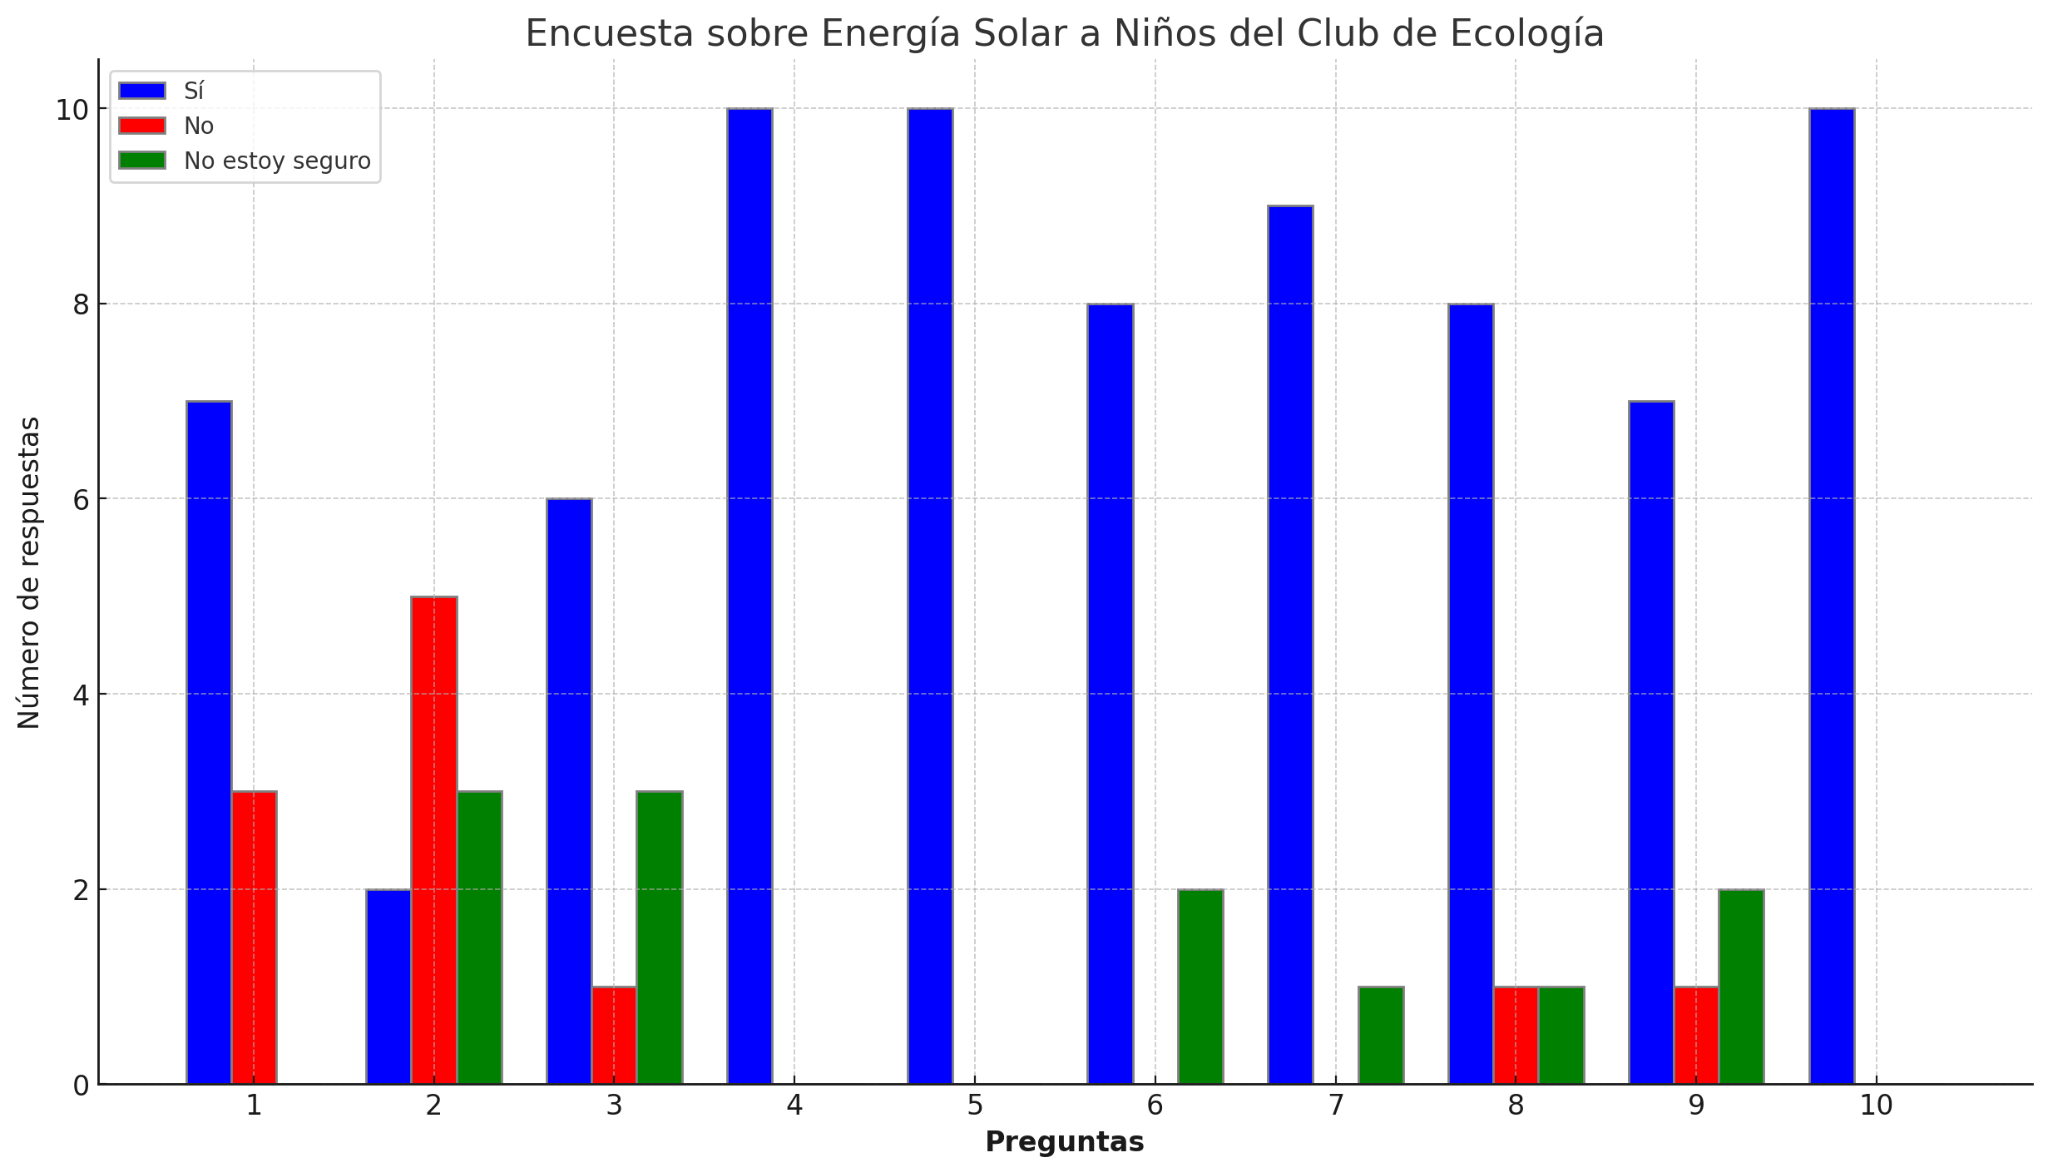
\includegraphics[width=0.5\textwidth]{imagenes/graph.png}
\end{center}
\newpage
\section{Conclusión}
El acceso al agua potable es un desafío que ha acompañado a la humanidad a lo largo de la historia. En la actualidad, la crisis hídrica requiere soluciones innovadoras que permitan garantizar la disponibilidad y calidad del recurso de manera sostenible. En este sentido, Aqua Solar representa una propuesta tecnológica viable y eficaz, capaz de integrar energía solar en sistemas de abastecimiento de agua para comunidades con infraestructura deficiente.

Los hallazgos del proyecto demuestran que la energía fotovoltaica es una alternativa eficiente para la gestión del agua, reduciendo costos operativos y minimizando el impacto ambiental. A través de su implementación, se espera beneficiar a miles de personas, mejorando su calidad de vida y reduciendo los riesgos sanitarios asociados al consumo de agua no potable.

El impacto de Aqua Solar no se limita a sus beneficiarios directos, sino que sienta las bases para el desarrollo de nuevas estrategias de abastecimiento hídrico sostenible. A futuro, se plantea la posibilidad de expandir el proyecto a nivel regional, incorporando avances tecnológicos en almacenamiento de energía y automatización de los sistemas de distribución.

En definitiva, Aqua Solar demuestra que la combinación de tecnología y sostenibilidad es clave para enfrentar los retos actuales del acceso al agua. Su implementación no solo representa una solución innovadora, sino que también marca un precedente en la búsqueda de modelos sustentables que puedan replicarse a nivel global.

\newpage
\nocite{*}
\bibliography{referencias}  % Sin la extensión .bib
\bibliographystyle{apacite} % Estilo APA
\newpage
\section{Anexos}

\subsection{Logo}
\begin{center}
      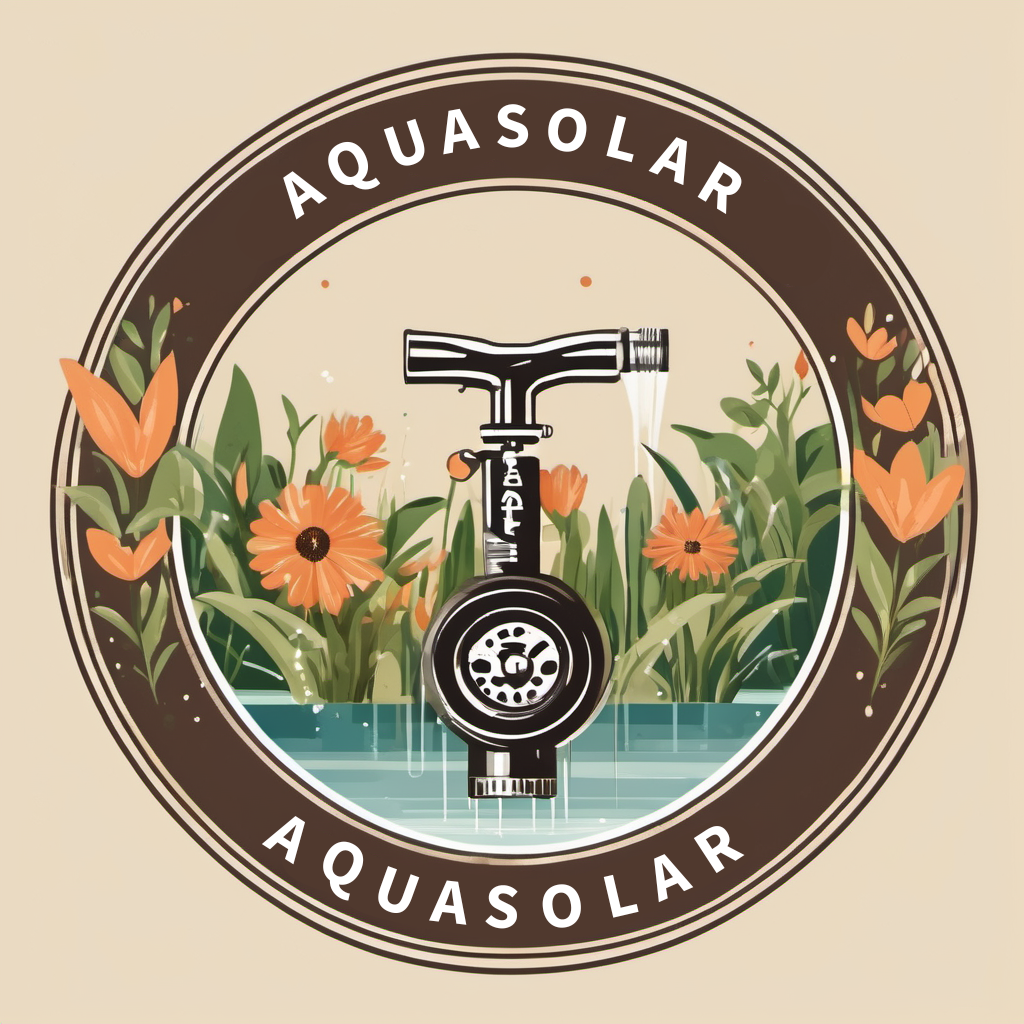
\includegraphics[width=0.5\textwidth]{imagenes/logo.png}
\end{center}

\subsection{Actividades}
\begin{itemize}
      \item \textbf{Preparación del terreno para la instalación del sistema de riego.}
            \begin{center}
                  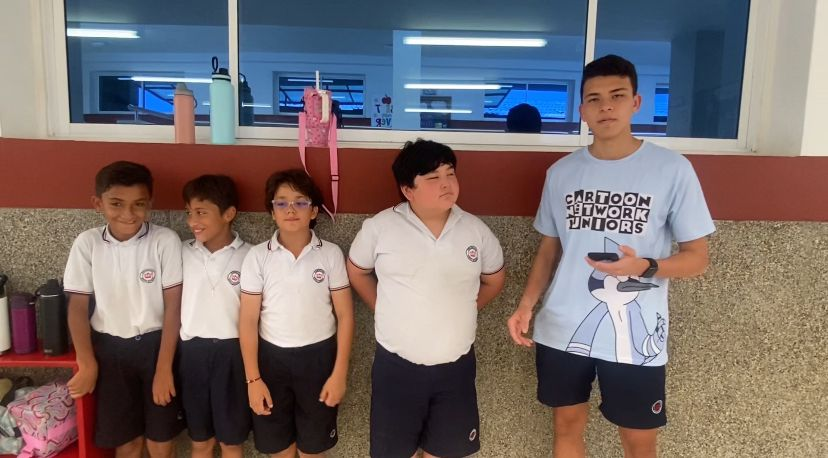
\includegraphics[width=0.5\textwidth]{imagenes/actividad1.jpg}
            \end{center}

      \item \textbf{Reforma del sistema de riego en la huerta escolar.}
            \begin{center}
                  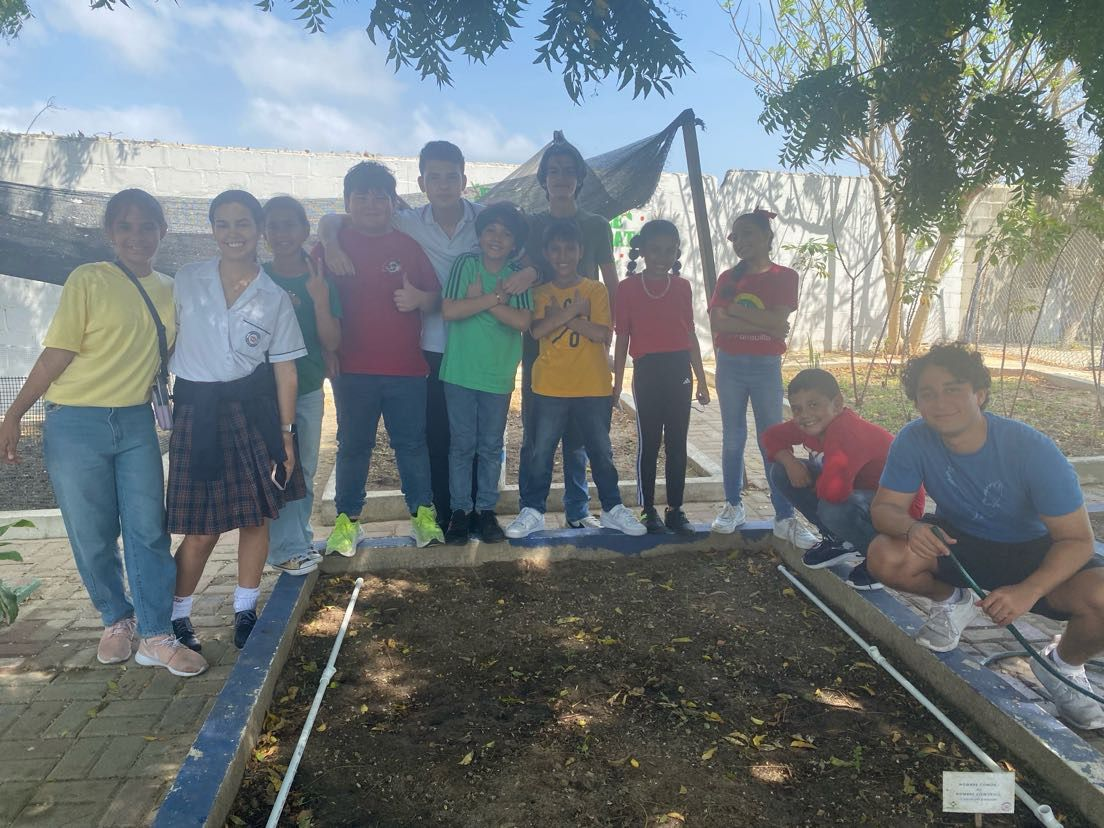
\includegraphics[width=0.5\textwidth]{imagenes/actividad2.jpg}
            \end{center}

      \item \textbf{Participación del Club de Ecología de primaria en la reforma del sistema de riego.}
            \begin{center}
                  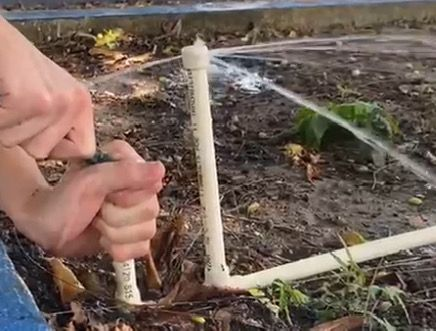
\includegraphics[width=0.5\textwidth]{imagenes/sprinkler.jpg}
            \end{center}
            \newpage
      \item \textbf{Instalación de la tubería y sistema de riego en la huerta.}
            \begin{figure}[h!]
                  \centering
                  \begin{minipage}[b]{0.48\textwidth}
                        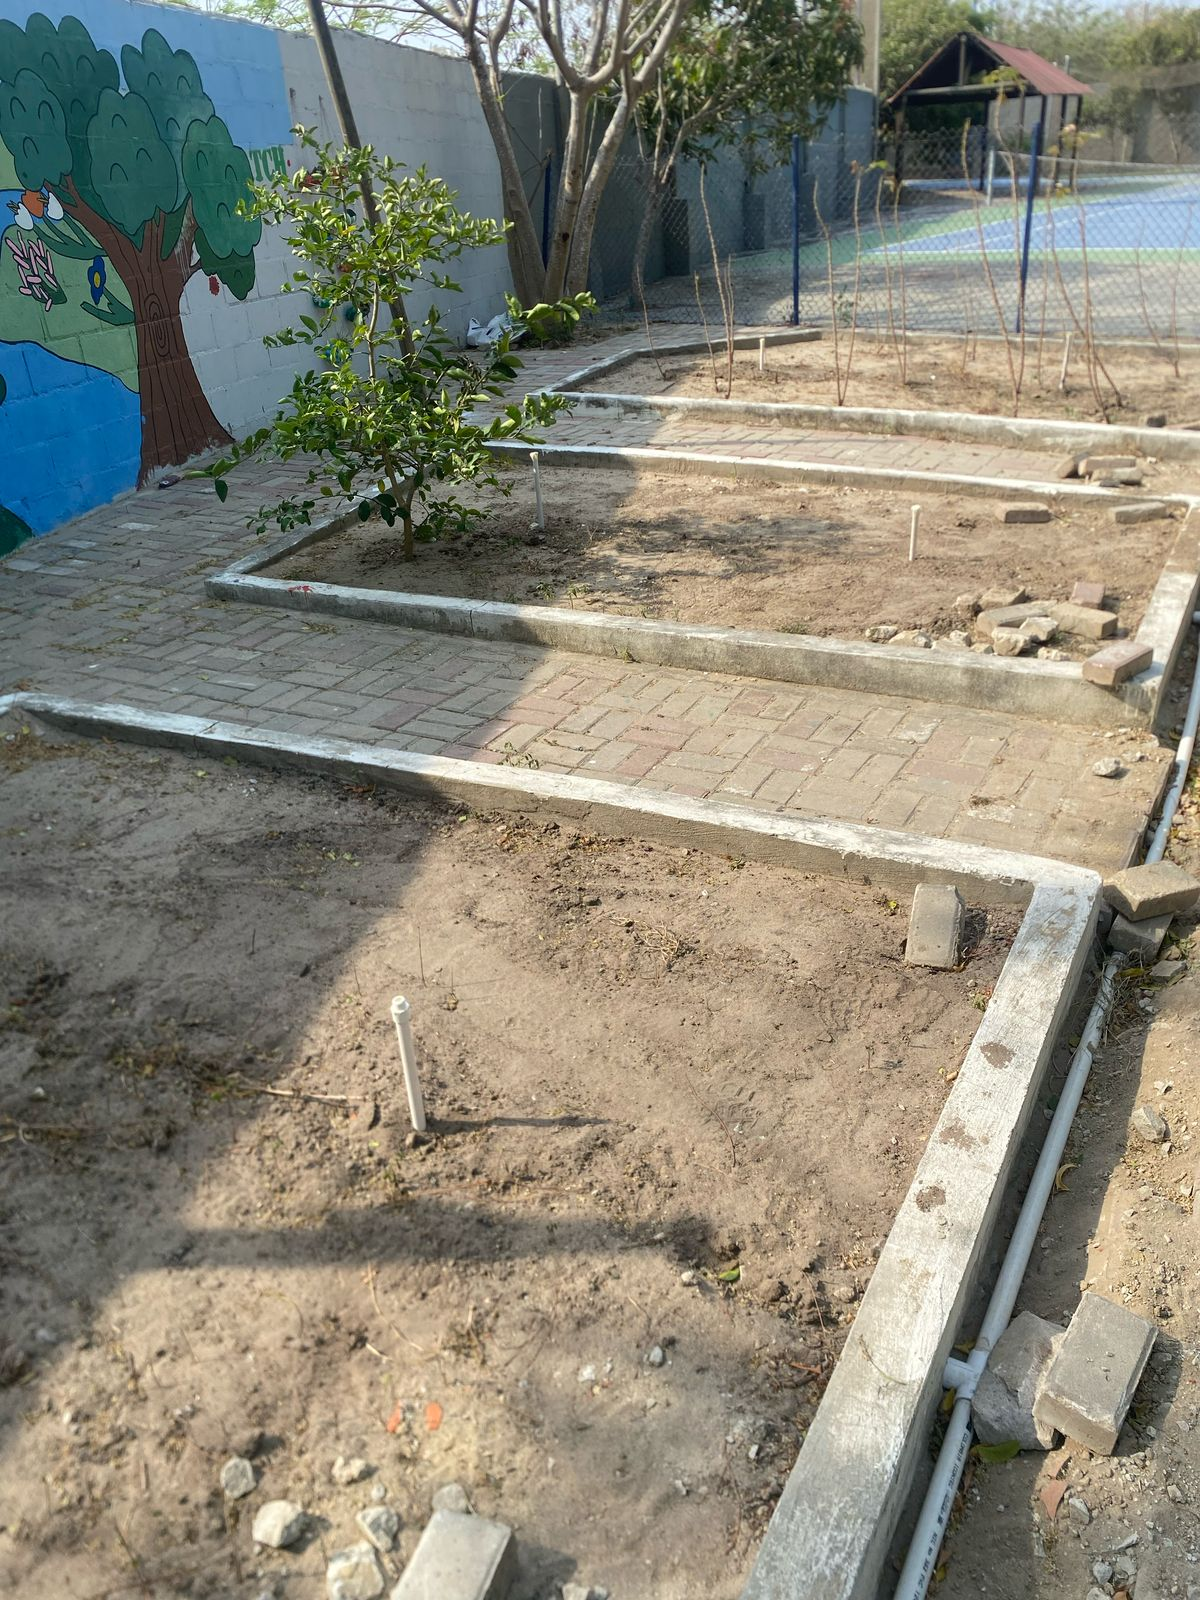
\includegraphics[width=\textwidth]{imagenes/sprinkler2.jpg}
                  \end{minipage}
                  \hfill
                  \begin{minipage}[b]{0.48\textwidth}
                        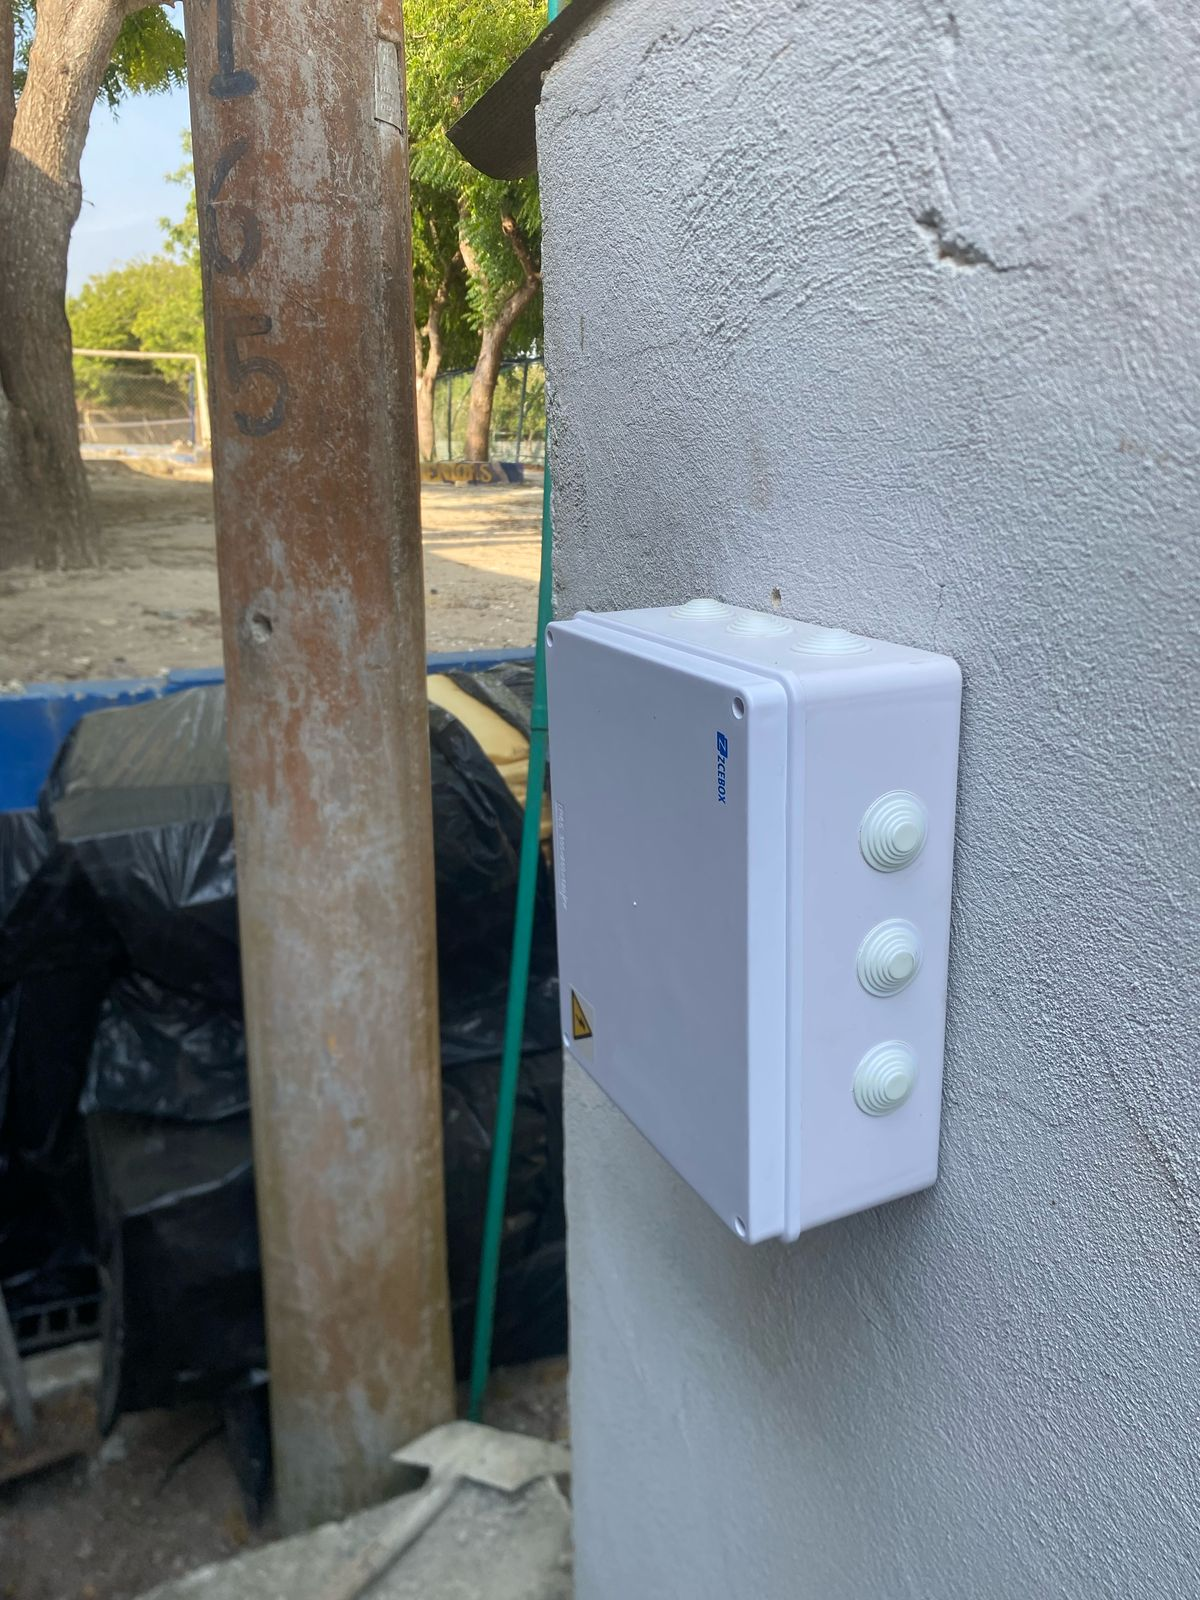
\includegraphics[width=\textwidth]{imagenes/box.jpg}
                  \end{minipage}
            \end{figure}

\end{itemize}

\subsection{Materiales Utilizados}
\begin{itemize}
      \item \textbf{Arduino Nano}
            \begin{center}
                  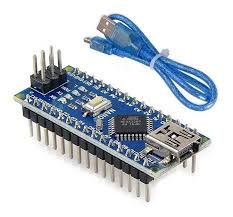
\includegraphics[width=0.3\textwidth]{imagenes/arduino.jpg}
            \end{center}

      \item \textbf{Panel Solar}
            \begin{center}
                  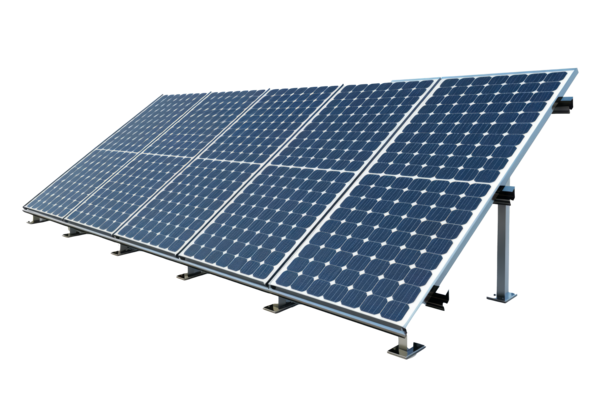
\includegraphics[width=0.3\textwidth]{imagenes/pane.png}
            \end{center}

      \item \textbf{Controlador de carga}
            \begin{center}
                  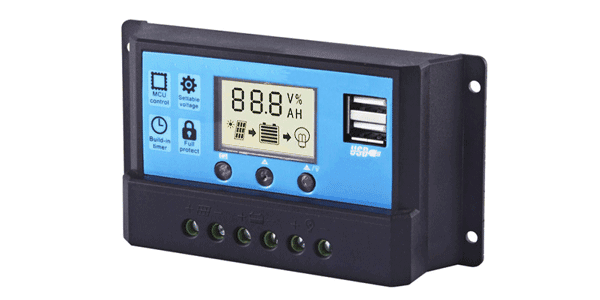
\includegraphics[width=0.3\textwidth]{imagenes/controlaor.png}
            \end{center}

      \item \textbf{Driver de motor}
            \begin{center}
                  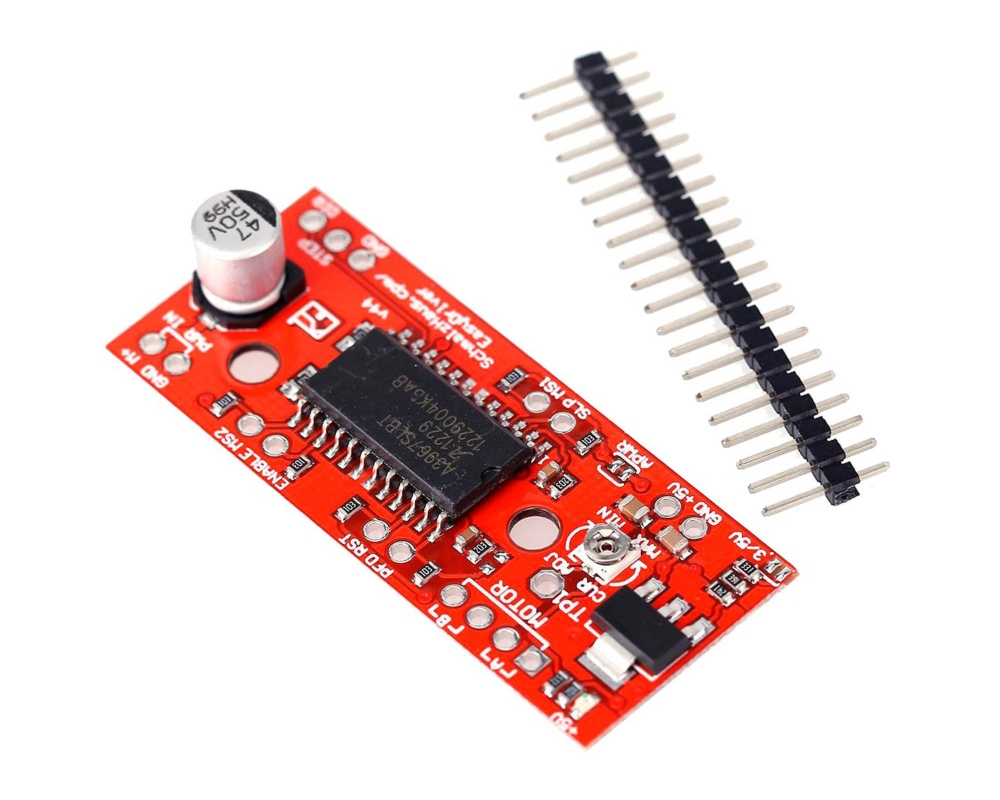
\includegraphics[width=0.3\textwidth]{imagenes/motor.png}
            \end{center}

      \item \textbf{Inversor Truper - 200W}
            \begin{center}
                  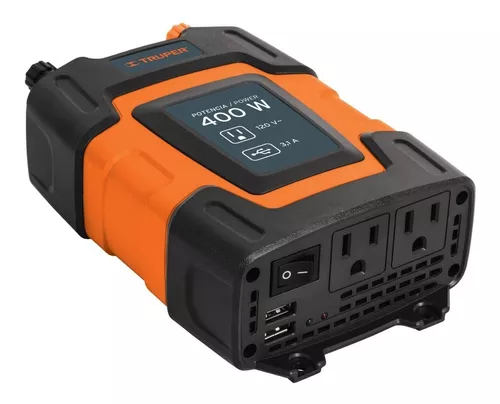
\includegraphics[width=0.3\textwidth]{imagenes/inversor.png}
            \end{center}

      \item \textbf{Electroválvula}
            \begin{center}
                  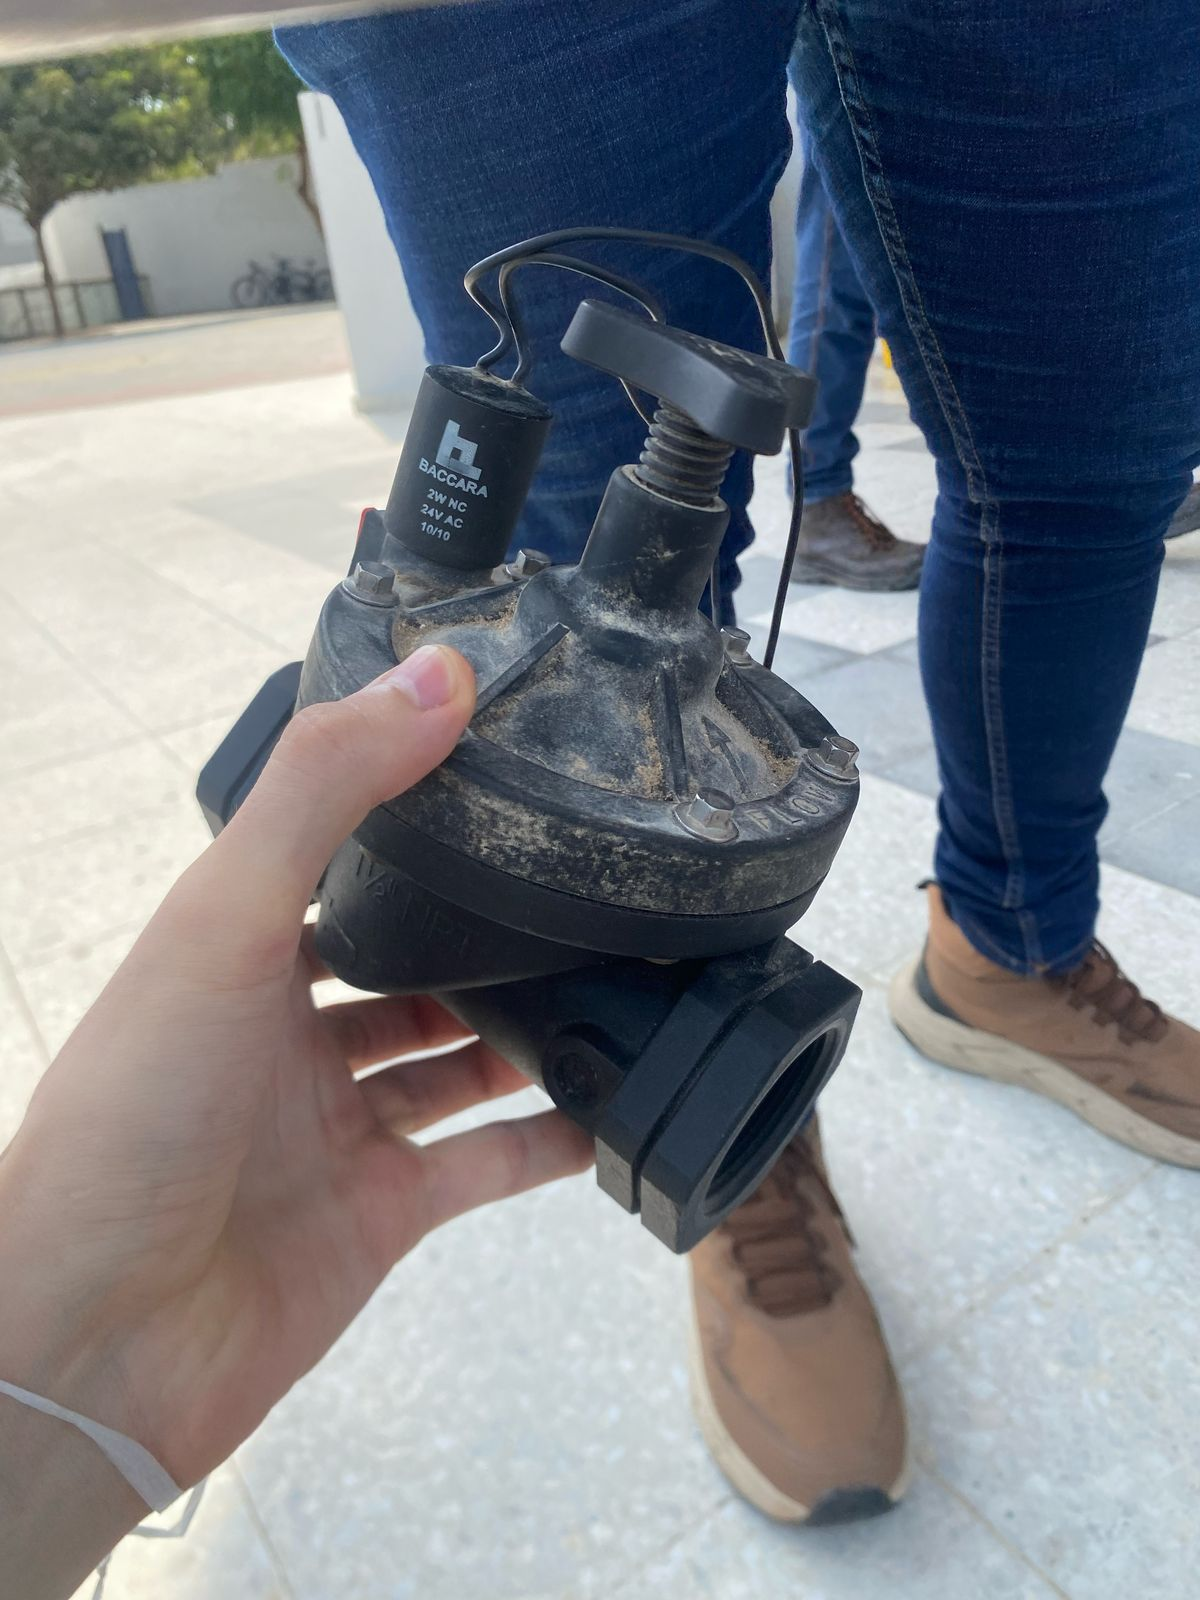
\includegraphics[width=0.3\textwidth]{imagenes/electrovalve2.jpg}
            \end{center}

      \item \textbf{Caja IP-65}
            \begin{center}
                  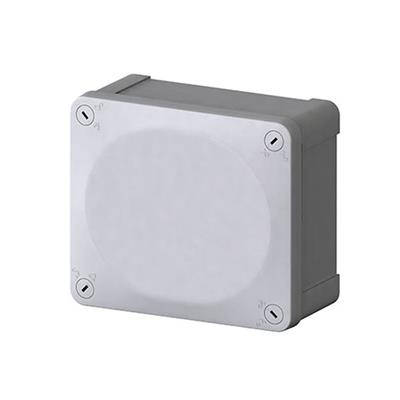
\includegraphics[width=0.3\textwidth]{imagenes/caja.png}
            \end{center}

      \item \textbf{Protoboard}
            \begin{center}
                  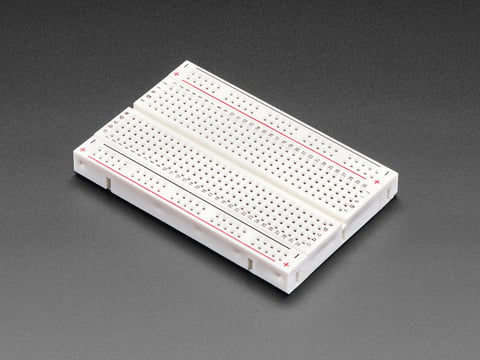
\includegraphics[width=0.3\textwidth]{imagenes/breadboard.png}
            \end{center}

      \item \textbf{Batería 12V 5Ah/20HR}
            \begin{center}
                  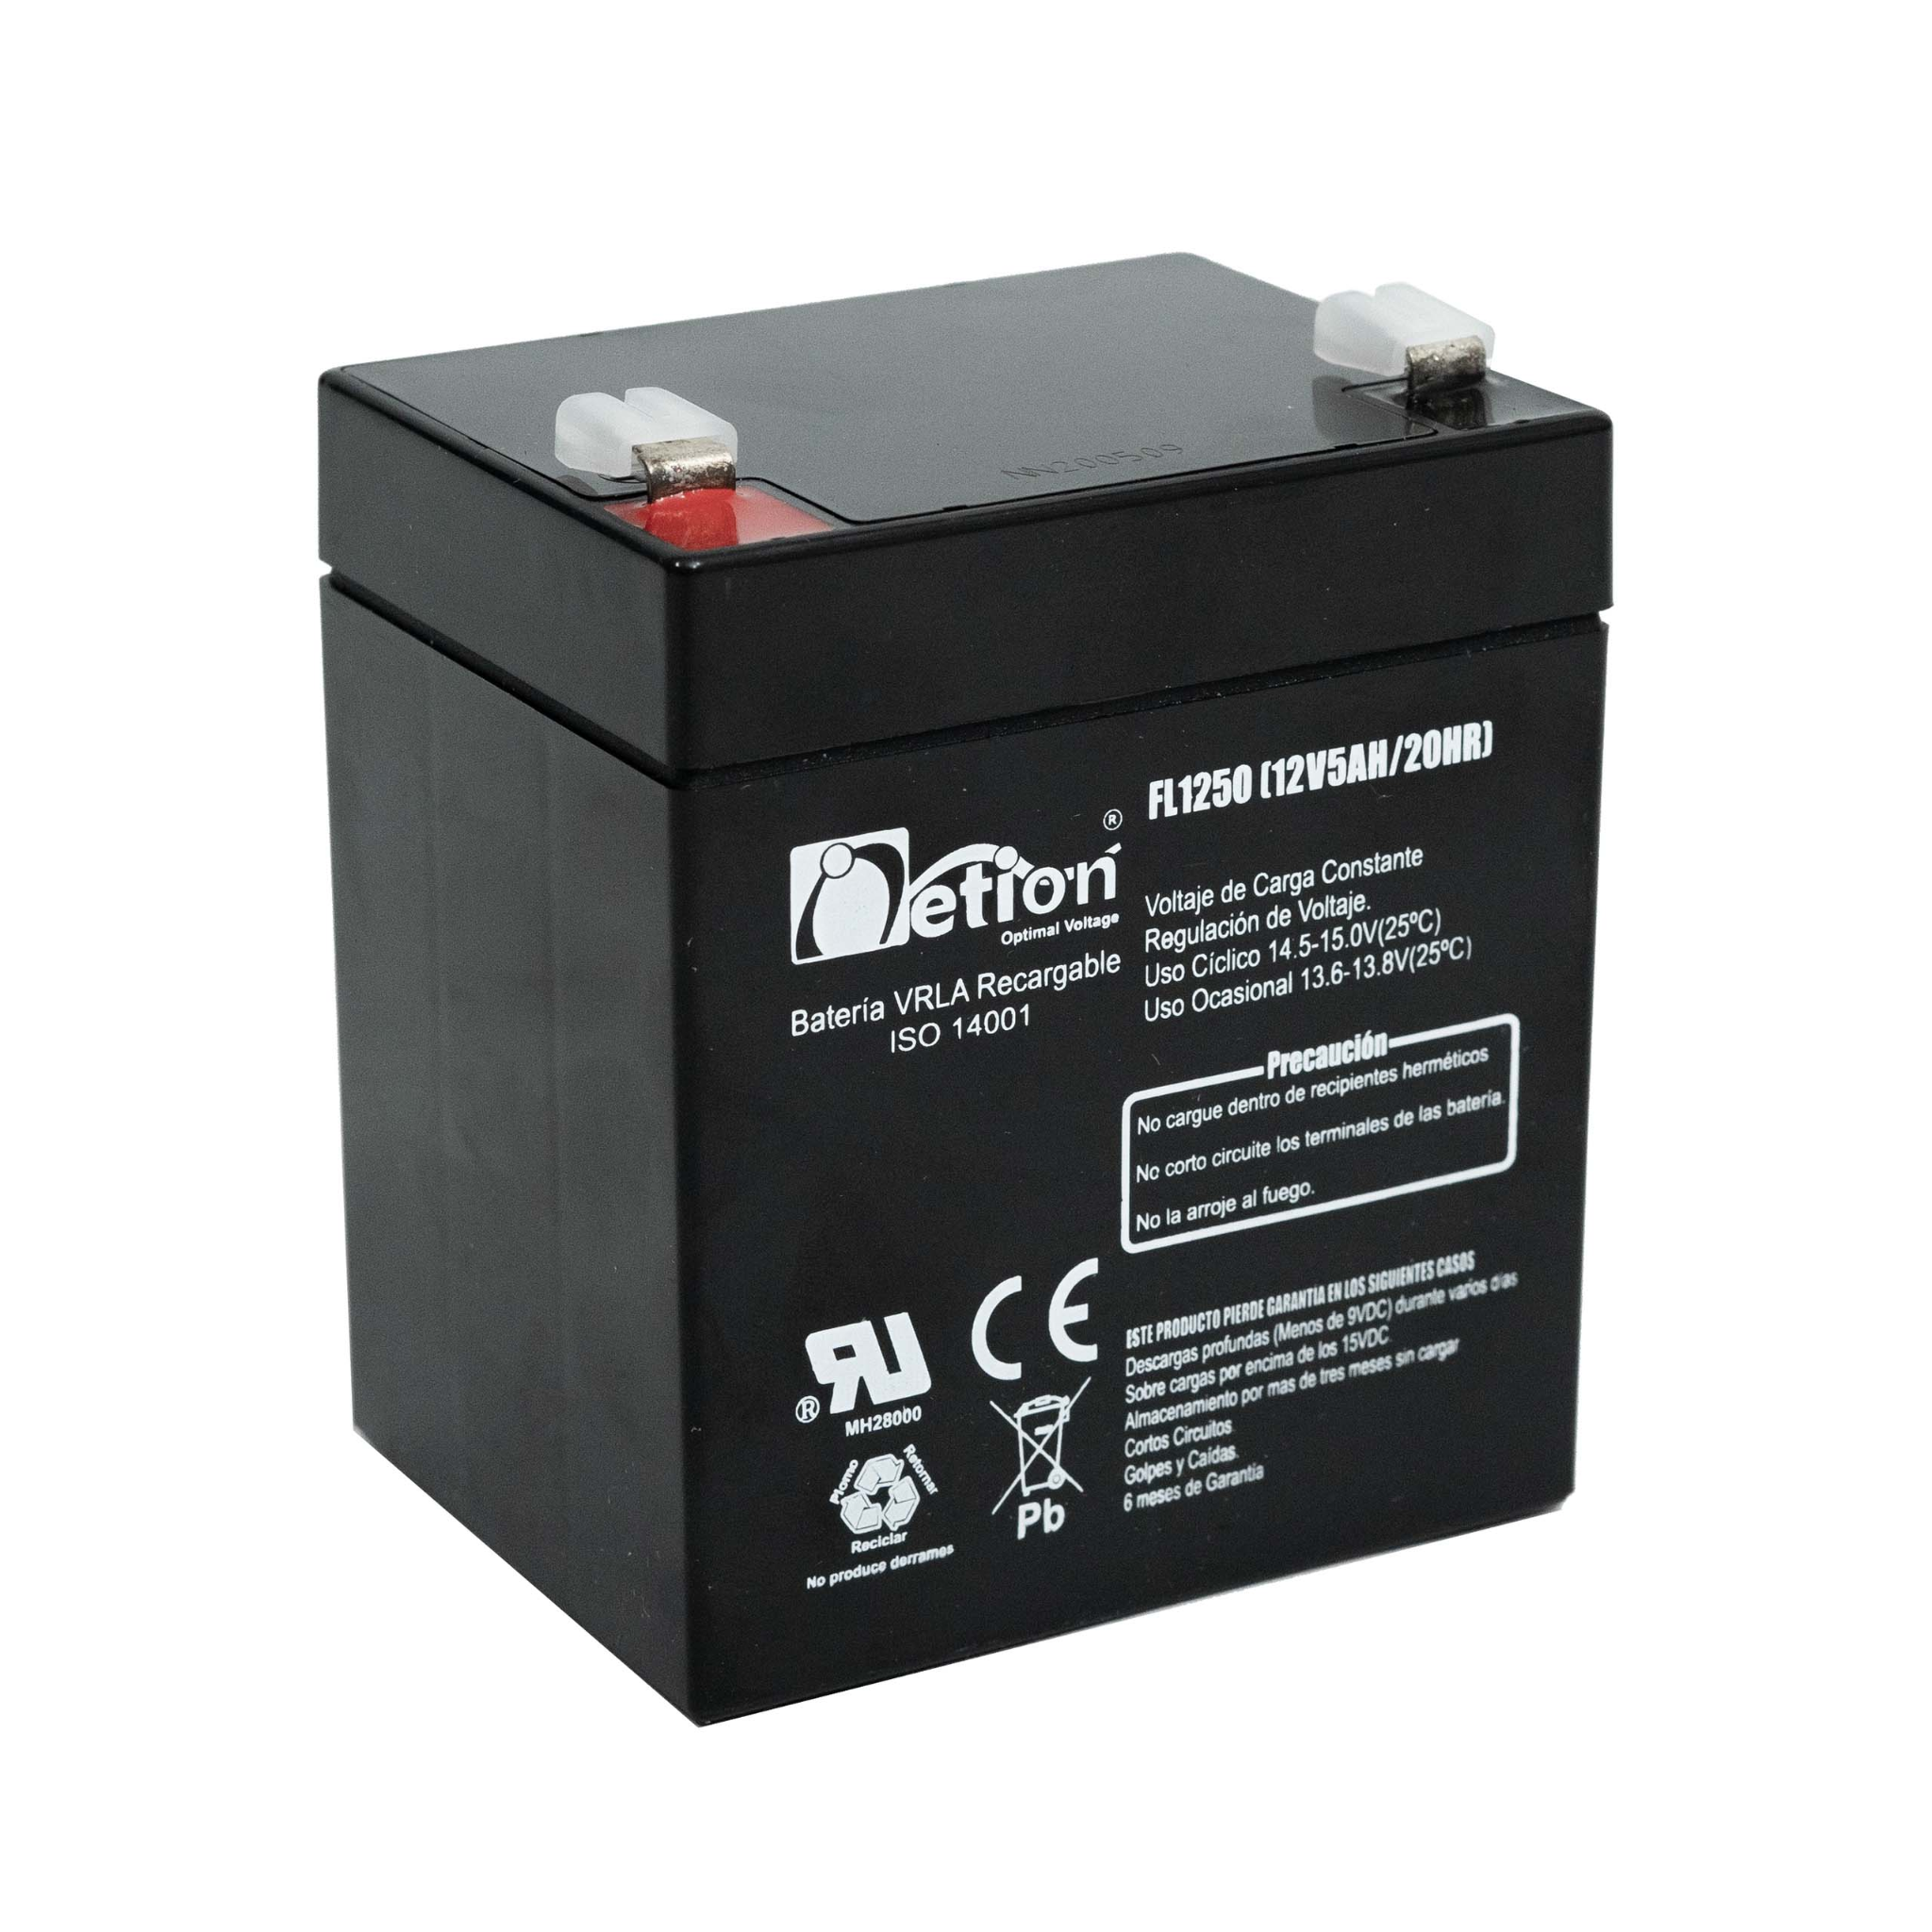
\includegraphics[width=0.3\textwidth]{imagenes/bateria.png}
            \end{center}
\end{itemize}

\end{document}